\documentclass[a4paper]{article}
\linespread{1.6}
\usepackage{enumerate}
\usepackage{geometry}
\usepackage{setspace}
\usepackage{amsmath}
\usepackage{amssymb}
\usepackage{cite}
\usepackage[pdftex]{graphicx}
\usepackage{float}
\usepackage{subfigure}
\usepackage{listings}
\geometry{left=1.4cm,right=1.4cm,top=2.5cm,bottom=2.5cm}

\begin{document}
\begin{spacing}{2.0}
\begin{flushleft}\begin{huge}EEL5840 Fundamental Machine Learning   Homework 5\end{huge}\end{flushleft}
\begin{flushright}\begin{Large} Hudanyun Sheng \end{Large}\end{flushright}

%\Large{All the code used are attached at the end of this report.}

Before performing classification algorithms, several  observations on the given data set is made: 
\begin{enumerate}
\item The five features except for those two describing gender are approximately Gaussian distributed:

\begin{figure}[htbp] 
\centering
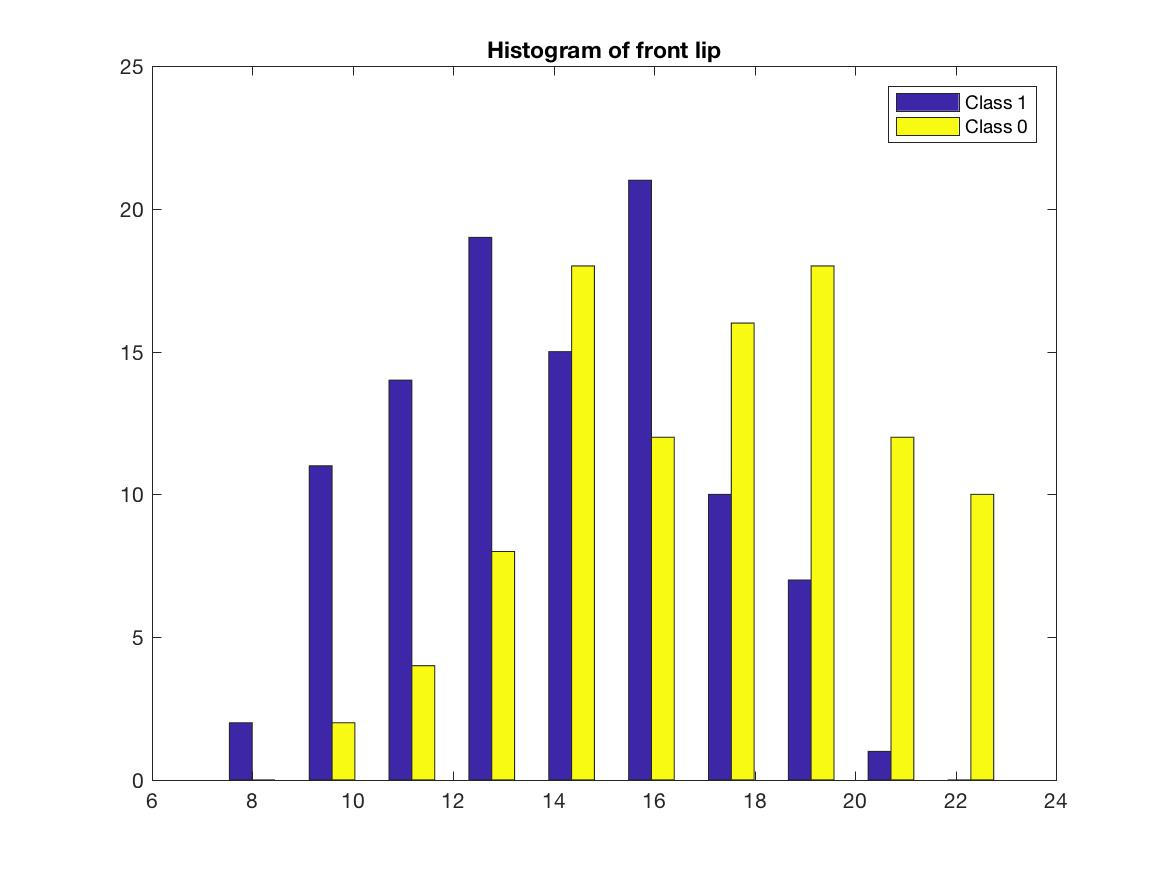
\includegraphics[width=1.5in]{feature1.jpg} 
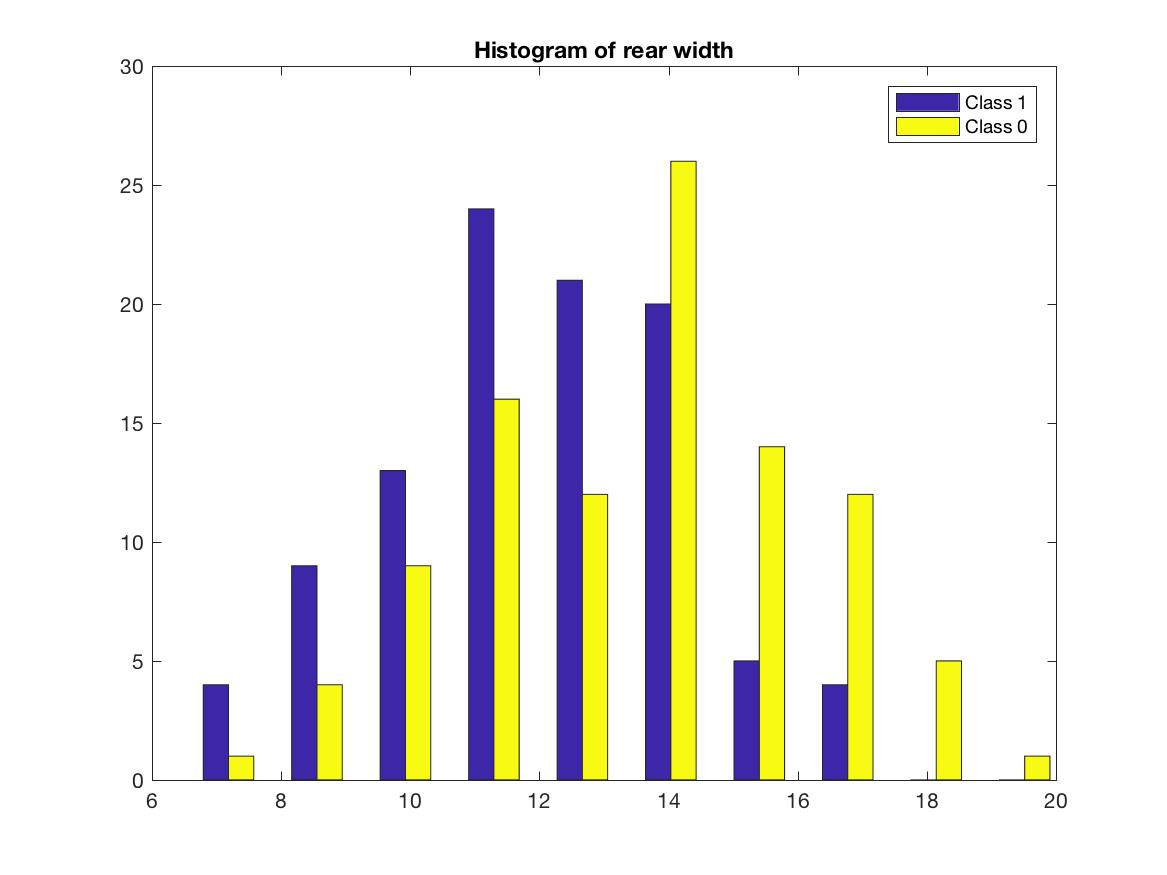
\includegraphics[width=1.5in]{feature2.jpg} 
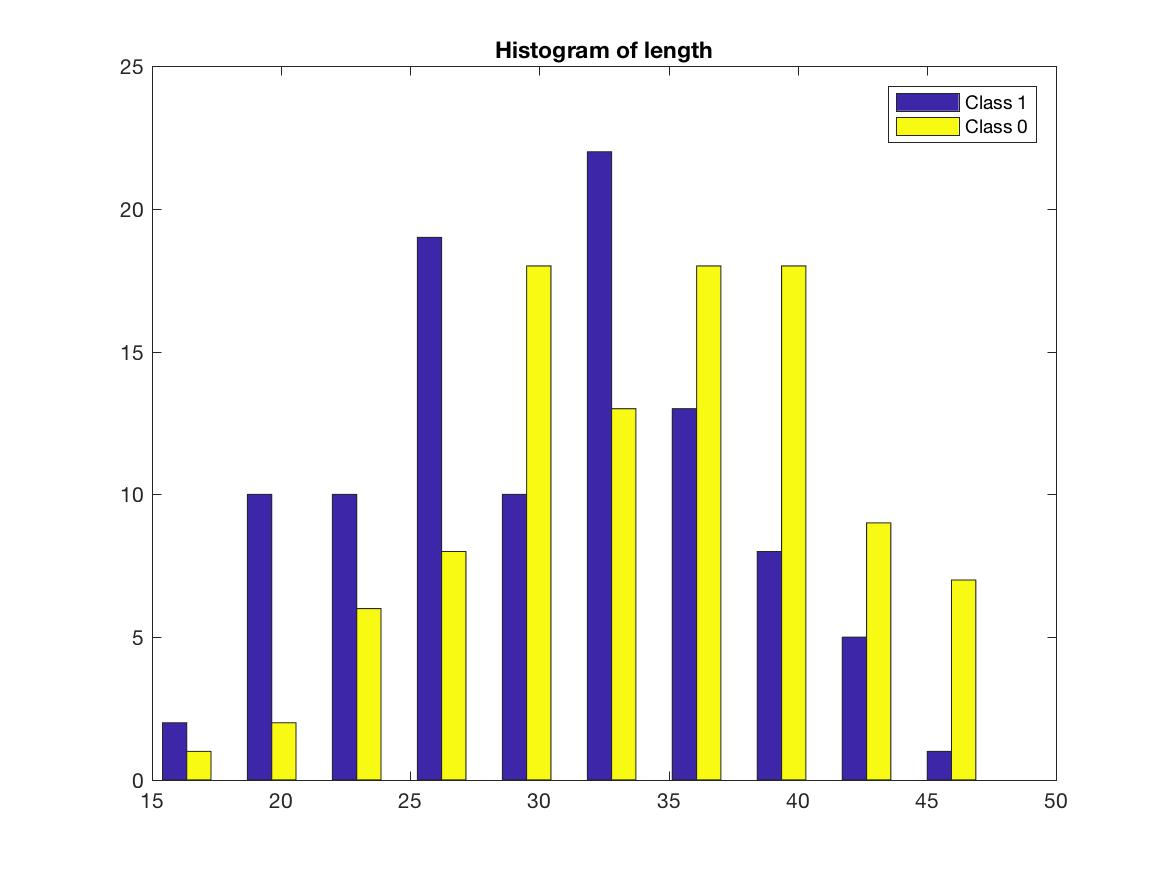
\includegraphics[width=1.5in]{feature3.jpg} 
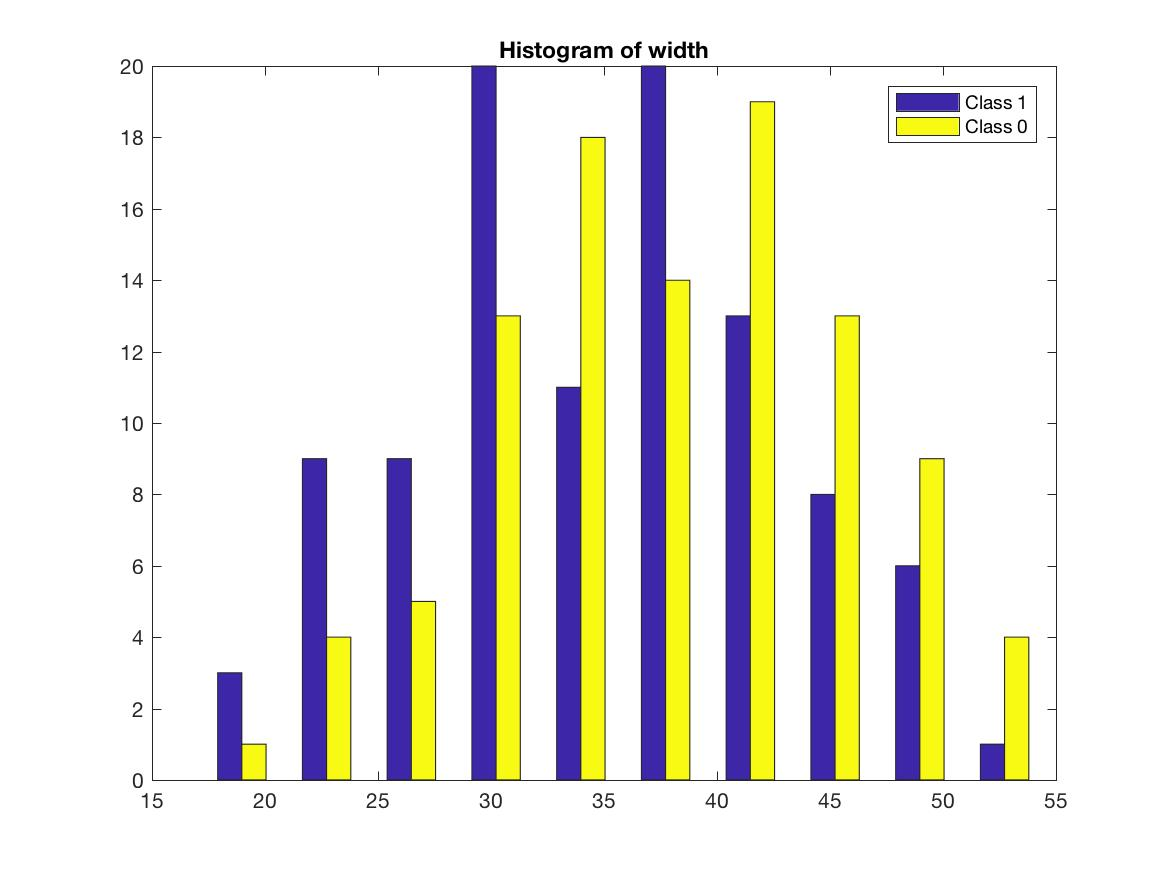
\includegraphics[width=1.5in]{feature4.jpg} 
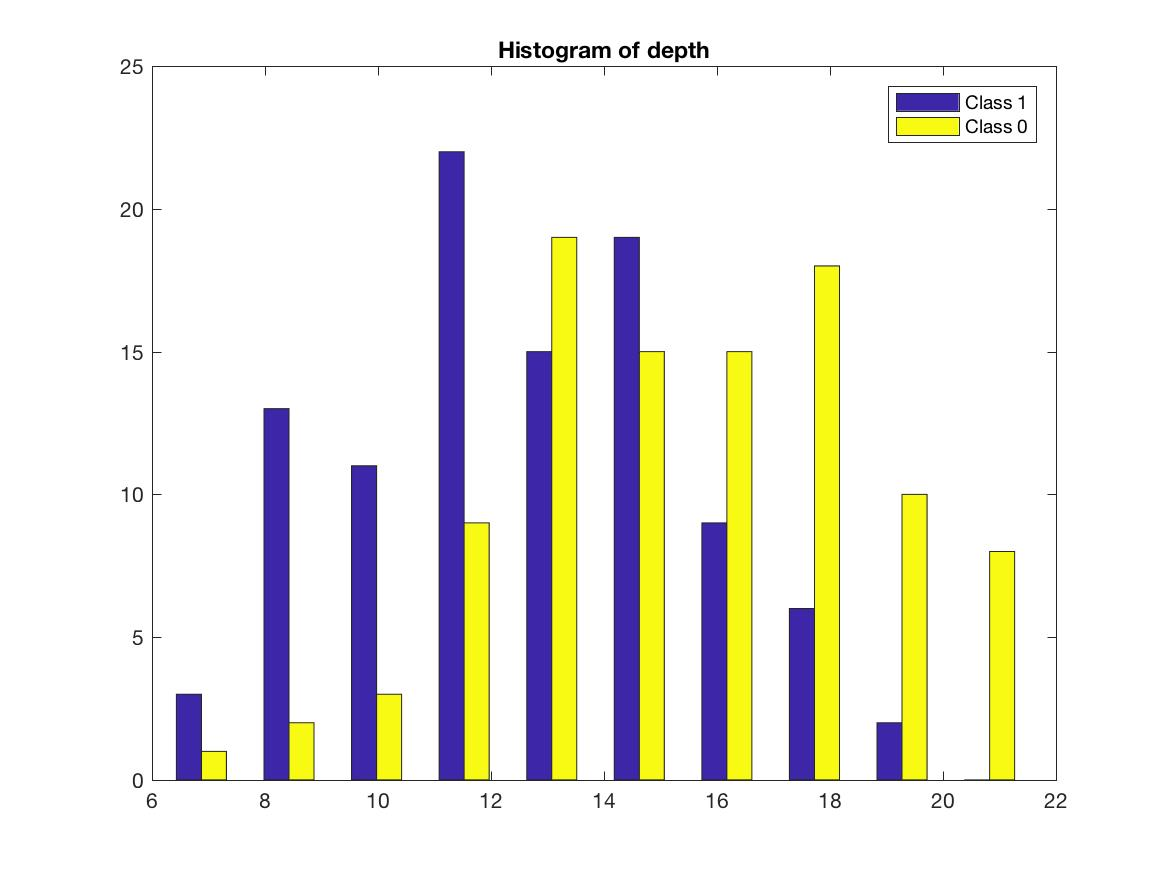
\includegraphics[width=1.5in]{feature5.jpg} 
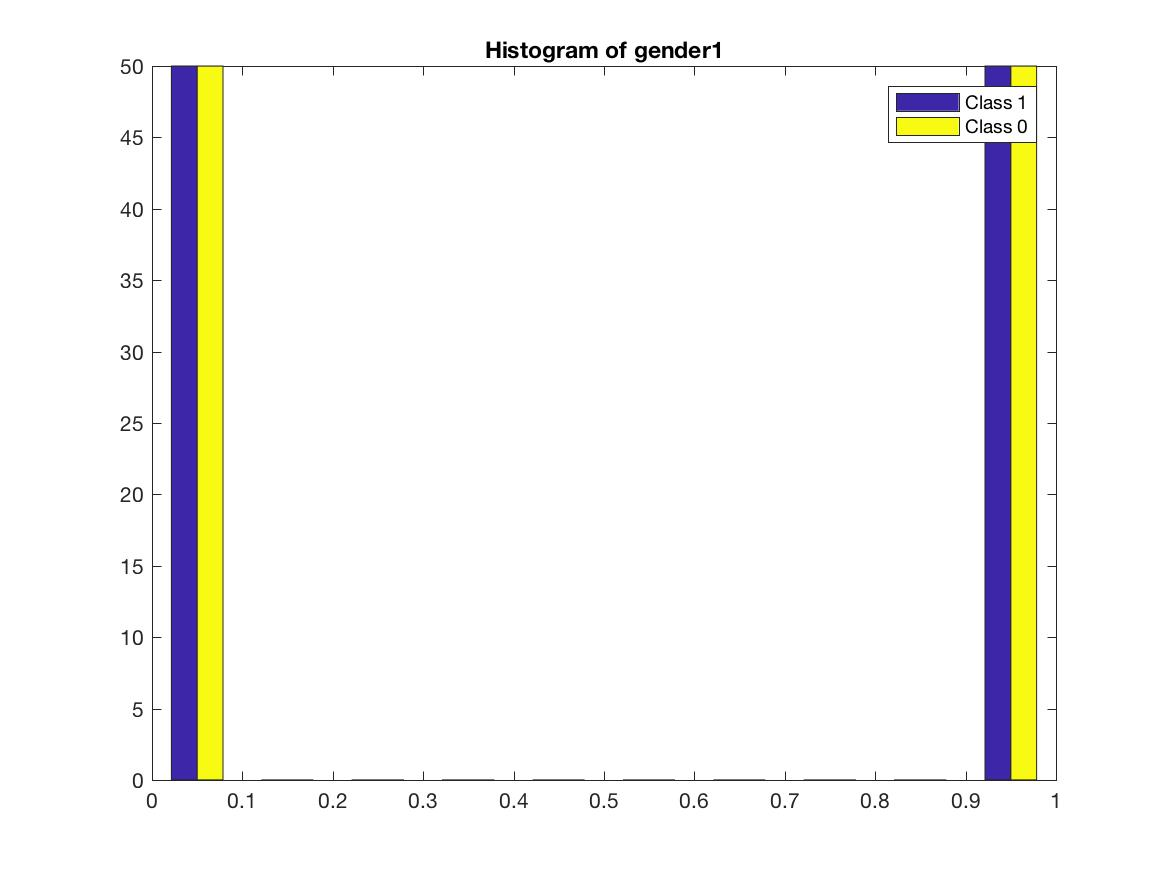
\includegraphics[width=1.5in]{feature6.jpg} 
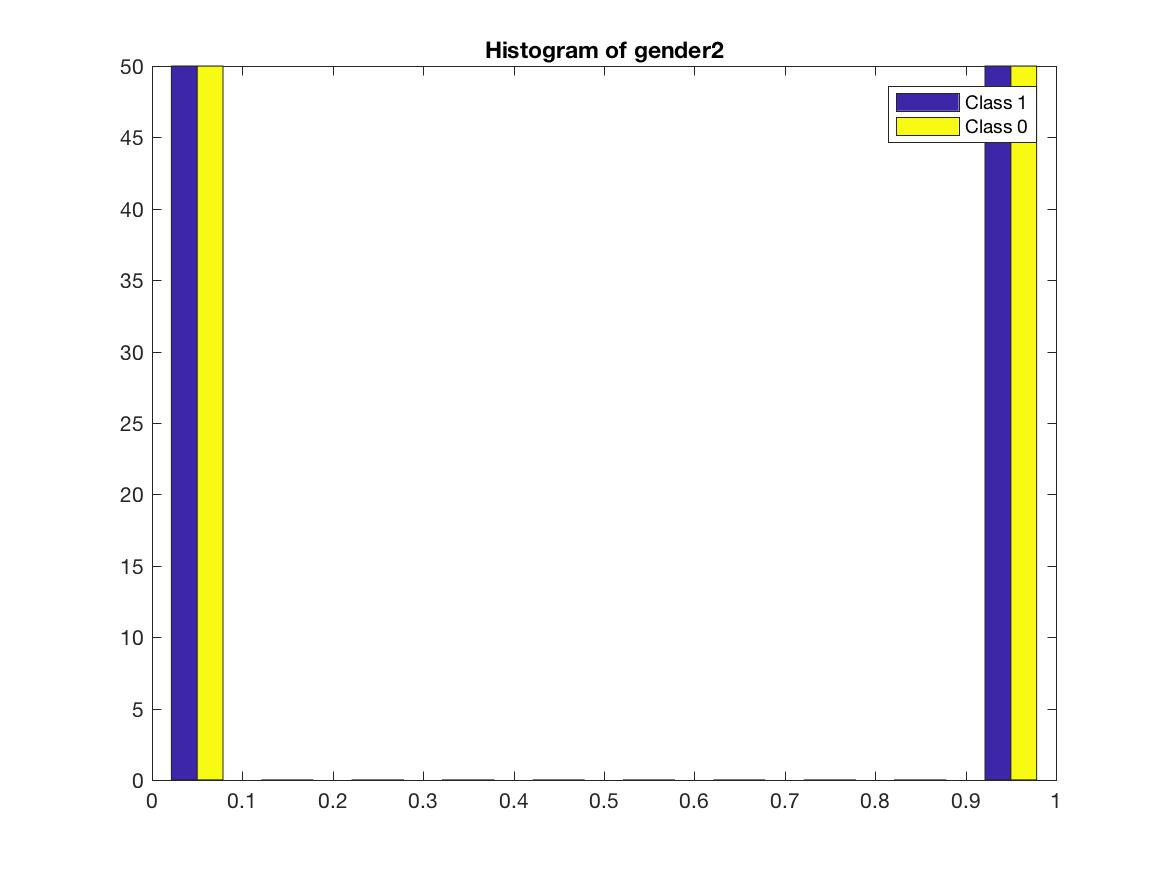
\includegraphics[width=1.5in]{feature7.jpg} 
\caption{Histogram of all features }\label{hist} 
\end{figure} 

When looking at the visualization of histogram of all the features, we see that for every feature, the data are approximately Gaussian distributed for each class.

\item The total number of instances in our data set is 200, 100 of them belong to class 1, 100 of them belong to class 0.

\item With both of the methods, we are using $70 \%$ of data (the first 140 samples) as our training set, we can calculated that the prior probability based on training data for class 0 is 0.5143, and the prior probability for class 1 is 0.4857.

\item When calculating the covariance matrix on the whole data set, there appears a warning says that `` Matrix is close to singular or badly scaled. Results may be inaccurate", which means that the condition number is too large for this data set, in that case, a small number $\lambda$ should be added to the diagonal of the covariance matrix, or maybe feature selection should be tried.

\item The last two features seems redundant- if an instance is ``male", it is obvious not ``female".\\

\end{enumerate}

\newpage
\paragraph{\huge\textbf{ Bayes classifier\\} }
\normalsize
The code is attached at the end of this report.\\
\begin{enumerate}
\item
Even if no regularization term $\lambda$ is not added to the covariance matrix, there would be warning `` Matrix is close to singular or badly scaled. Results may be inaccurate", but the detection procedure works well. The \textbf{confusion matrix} for the train set is 
$$\begin{bmatrix}
68 & 0 \\
0 & 72 
\end{bmatrix}$$
We can conclude that the detection rate for train set is $100\%$

The \textbf{confusion matrix} for the test set is 
$$\begin{bmatrix}
32 & 0 \\
0 & 28 
\end{bmatrix}$$
We can conclude that he detection rate for test set is $100\%$

The \textbf{confusion matrix} for the entire set is 
$$\begin{bmatrix}
100 & 0 \\
0 & 100 
\end{bmatrix}$$
We can conclude that the detection rate for entire set is $100\%$. And based on MATLAB, the amount of time needed to classify the entire dataset is 0.251246 seconds.\\

\item
If add a regularization term $\lambda = 0.1$, there is no warning regarding the covariance, the confusion matrices remain the same, and the time needed to classify the entire dataset becomes shorter, though changes with different experiments, is around 0.012197.

\item
When the last feature or the sixth feature is removed, the detection result remains unchanged - with same confusion matrices and no regularization term needed. The time needed to classify the entire dataset has little changes, i.e. 0.009406 seconds. 

\item
When both of the 6th and 7th features are removed, i.e. only the first five features are used, I still got the classify result $100\%$ correct, thus the confusion matrices did not change, and the time needed to classify did not change a lot.
\end{enumerate}

\newpage
\paragraph{\huge\textbf{ Linear discriminant analysis\\} }
\normalsize
The code is attached at the end of this report.
\begin{enumerate}
\item If all features are kept, then there is still a problem regarding the condition number of the covariance matrix, so a regularization term is needed, i.e. I use $\lambda = 0.1$. And  in this way, the value of threshold T should be set to 0 to have 100\% classification result. The time needed to build the model (i.e. calculate the values of $\mu$ and $\sigma$) is 0.001732seconds, and the time needed to classify the entire data set is 0.010502 seconds. The \textbf{confusion matrix} for the train set is 
$$\begin{bmatrix}
68 & 0 \\
0 & 72 
\end{bmatrix}$$
We can conclude that the detection rate for train set is $100\%$

The \textbf{confusion matrix} for the test set is 
$$\begin{bmatrix}
32 & 0 \\
0 & 28 
\end{bmatrix}$$
We can conclude that he detection rate for test set is $100\%$

The \textbf{confusion matrix} for the entire set is 
$$\begin{bmatrix}
100 & 0 \\
0 & 100 
\end{bmatrix}$$
\item
If we keep only 6 features, then the regularization term is not needed. The value of threshold T should be set between [-31, -19] to have 100\% correct classification ratio. So that the confusion matrices remain unchanged, and the time needed to classify entire dataset is 0.007403 seconds.\\
If the threshold value is chosen to be -18, then there is a misclassification instance occur in the test on the training set. The \textbf{confusion matrix} for the train set is 
$$\begin{bmatrix}
67 & 1 \\
0 & 72 
\end{bmatrix}$$
The \textbf{confusion matrix} for the test set is 
$$\begin{bmatrix}
32 & 0 \\
0 & 28 
\end{bmatrix}$$
We can conclude that he detection rate for test set is $100\%$

The \textbf{confusion matrix} for the entire set is 
$$\begin{bmatrix}
99 & 1 \\
0 & 100 
\end{bmatrix}$$
We can see that there is a data point which is actually belong to class 0 but is predicted to be belong to class 1.
\end{enumerate}

Here are some comparisons and summaries of the discussion above:
\begin{figure}[htbp]
\centering 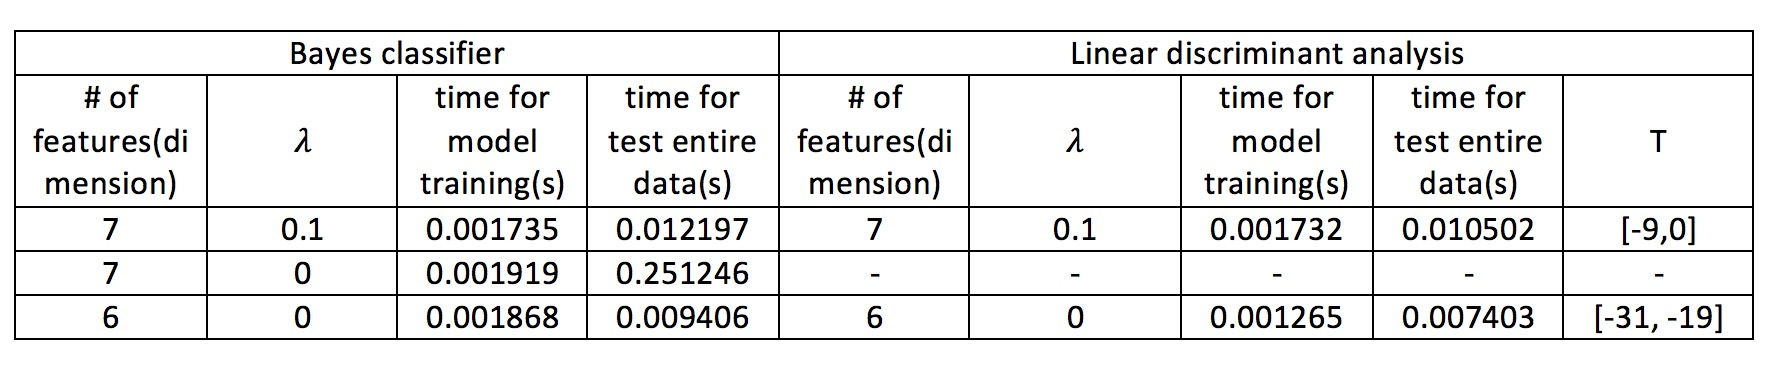
\includegraphics[width = 7in]{comparison.jpg}
\end{figure}

\large{Summaries:} 
\normalsize
\begin{enumerate}
\item The training part are the same for both of the methods - we only need to calculation the mean and covariance matrix using the training data.

\item Generally speaking, the linear discriminant analysis is efficient and need less time to classify the entire data set once we already have the model built, which makes sense since the LDA method ignore the calculation of determinant but instead using a scalar. But the difference is not that obvious.

\item For this data set, two methods performs with little difference. While LDA needs some time to carefully pick the threshold value.
\end{enumerate}

\newpage
\paragraph{\huge\textbf{ MATLAB code used for this report\\} }
Below is the \textbf{script} for this report:
\begin{lstlisting}
clear; clc, close all, dbstop if error
crab = importdata('HW5_dataset.txt'); %import data - structure
label = crab.data(:,1);
text = [ {'front lip'} {'rear width'} {'length'} {'width'} {'depth'} ...
{'gender1'} {'gender2'}];
%% visulization
for idx_f = 1:7
    feature = crab.data(:,idx_f+1);
    figure, hist([feature(label == 1) feature(label == 0)])
    title( ['Histogram of ' text{idx_f}] ), legend('Class 1', 'Class 0')
    fig = gcf; saveas(fig, ['feature' num2str(idx_f) '.jpg'] )
end
%%
d = 7; %choose the dimension we want to keep, if d = 7, than all the features are used
data       = crab.data(:,2:d+1);
trainset   = crab.data(1:140, 2:d+1);
trainlabel = crab.data(1:140,1);
testset    = crab.data(141:end, 2:d+1);
testlabel  = crab.data(141:end, 1);
confu_M    = zeros(2,2);
lambda     = 0.1;
%% train (the same using Bayes classifier or Linear discriminant analysis)
for j = 1:2
    index{1,j} = find(trainlabel==j-1);
    n{1,j} = length(index{1,j});
    prior{1,j} = n{1,j}/length(trainlabel);
    mu{1,j} = mean(trainset(index{1,j},:));
    sigma{1,j} = ((trainset(index{1,j},:)-mu{1,j})'*(trainset(index{1,j},:)...
    -mu{1,j}))/n{1,j}+lambda*eye(d);
end

%% test using Bayes classifier
%% on train set
label_predict_train = Bayes_test( trainset, mu, sigma, d, prior );
[ ratio_misclass_train, confu_M_train] ...
= computeConfusionM( label_predict_train, trainlabel );
disp('Confusion matrix for test on train set is ' )
disp(confu_M_train)
%% on test set
label_predict_test = Bayes_test( testset, mu, sigma, d, prior );
[ ratio_misclass_test, confu_M_test] ...
= computeConfusionM( label_predict_test, testlabel );
disp('Confusion matrix for test on test set is ')
disp(confu_M_test)
%% on entire dataset
tic 
label_predict_entire = Bayes_test( data, mu, sigma, d, prior );
toc
[ ratio_misclass_entire, confu_M_entire] ...
= computeConfusionM( label_predict_entire, label );
disp('Confusion matrix for test on entire set is ')
disp(confu_M_entire)

%% test using Linear Discriminant Analysis
T = -9; % set the value of threshold
% on train set
label_predict_train = LDA_test( trainset, mu, sigma, T );
[ ratio_misclass_train, confu_M_train] ...
= computeConfusionM( label_predict_train, trainlabel );
disp('Confusion matrix for test on train set is ')
disp(confu_M_train)
% on test set
label_predict_test = LDA_test( testset, mu, sigma, T );
[ ratio_misclass_test, confu_M_test] = computeConfusionM( label_predict_test, testlabel );
disp('Confusion matrix for test on test set is ')
disp(confu_M_test)
%% on entire set
tic
label_predict_entire = LDA_test( data, mu, sigma, T );
toc
[ ratio_misclass_entire, confu_M_entire] = computeConfusionM( label_predict_entire, label );
disp('Confusion matrix for test on entire set is ')
disp(confu_M_entire)
\end{lstlisting}
\Large{This script contains three \textbf{functions}, which are attached below:}
\normalsize
\begin{enumerate}
\item Function to perform \textbf{Bayes test:} 
\begin{lstlisting}
function [ label_predict ] = Bayes_test( data, mu, sigma, d, prior )
%Function of bayes test based on models already have
%	input: data
%	mu, siga from known model
%	d is the dimenssion of the data
%	prior is the prior probability
for idx = 1:size(data,1)
    for j = 1:2
        discriminant(idx,j) = -(1/2)*(data(idx,:)-mu{1,j})*inv(sigma{1,j})*(data(idx,:)-mu{1,j})'...
            -(d/2)*log(2*pi)-(1/2)*log(abs(det(sigma{1,j})))+log(prior{1,j});
    end 
    if discriminant(idx,1)>discriminant(idx,2)
        label_predict(idx,1) = 0;
    else
        label_predict(idx,1) = 1;
    end
end
end
\end{lstlisting}
\item Function to perform \textbf{Linear discriminant analysis} test to classify:
\begin{lstlisting}
function label_predict = LDA_test( data, mu, sigma, T )
%Function of LDA test based on models already have
%	input: data
%	mu, siga from known model
%	d is the dimenssion of the data
%	T is the threshold
for idx = 1:size(data,1)
	discriminant(idx,1) = sum((inv((sigma{1,2}+sigma{1,1})/2)*(mu{1,2}-mu{1,1})')...
	.*data(idx,:)')-(mu{1,1}*inv(sigma{1,1})*mu{1,1}' ...
	- mu{1,2}*inv(sigma{1,2})*mu{1,2}' + T)/2;%first way to calculate the ...
	%discriminant function
	discriminant(idx,1) = sum((inv(sigma{1,2}+sigma{1,1})*(mu{1,2}-mu{1,1})')...
	.*data(idx,:)') -(mu{1,1}*inv(sigma{1,1})*mu{1,1}' ...
	- mu{1,2}*inv(sigma{1,2})*mu{1,2}' + T)/4; %second way to calculate the ...
	%discriminant function
    if discriminant(idx,1) < 0
        label_predict(idx,1) = 0;
    else
        label_predict(idx,1) = 1;
    end
end
end
\end{lstlisting}
\item Function to compute the confusion matrix based on detection results:
\begin{lstlisting}
function [ ratio_misclass, confu_M ] = computeConfusionM( label_predict, label )
%Function to compute confusion matrix
%   Input:
%   predicted label: label predicted by the discrimint functions
%   true label: the ground truth from the data set
distance = label_predict - label;
ratio_misclass = length(find(distance ~= 0))/length(distance);
confu_M = zeros(2,2);
    [idx_0,~] = find(label == 0);
    for i = 1:length(idx_0)
        if label_predict(idx_0(i)) == 0
        confu_M(2,2) = confu_M(2,2)+1;
        else
        confu_M(2,1) = confu_M(2,1)+1;
        end
    end
    [idx_1,~] = find(label == 1);
    for i = 1:length(idx_1)
        if label_predict(idx_1(i)) == 1
        confu_M(1,1) = confu_M(1,1)+1;
        else
        confu_M(1,2) = confu_M(1,2)+1;
        end
    end
end
\end{lstlisting}
\end{enumerate}

\end{spacing}
\end{document}